\documentclass[12pt]{article}

\usepackage{sbc-template}
\usepackage{graphicx,url}
\usepackage[utf8]{inputenc}
\usepackage[brazil]{babel}
\usepackage{fancyvrb}
\usepackage{caption}
\usepackage{subcaption}

\newcommand\slsh{\char`\\}

\usepackage{hyperref}
\hypersetup{
    colorlinks=true,
    linkcolor=cyan,
    filecolor=blue,      
    urlcolor=cyan,
    citecolor=cyan,
}
 
\sloppy

\title{Projeto de análise experimental para comparação entre algoritmos de ordenação}

\author{Marcos Renan Krul}


\address{Universidade Estadual de Ponta Grossa (UEPG)}

\begin{document} 

\maketitle
     
\begin{resumo} 
 
 As técnicas de ordenação estão presentes em diversas aplicações e se caracterizam como um problema computacional muito bom para estudo da análise e projeto de algoritmos. O objetivo é realizar uma análise experimental entre três algoritmos de ordenação, a fim de definir em quais situações cada um deles possui uma vantagem. Os resultados validam o comportamento quadrático do Bubble sort em médio e pior caso, além da vantagem do quick sort em relação à ordenação digital para números com mais dígitos. 

\end{resumo}

\section{Introdução}

A ordenação de um conjunto de dados consiste, basicamente, no processo de rearranjo dos elementos, reorganizando-os em uma ordem ascendente ou descendente. Dessa forma, pode-se ordenar uma lista de valores numéricos de forma crescente, ou ainda uma lista de nomes em ordem lexicográfica (ordem alfabética). De forma prática, essa atividade está presente na maioria das aplicações onde os dados precisam ser pesquisados e recuperados, como dicionários, índices de livros, agendas telefônicas ou tabelas de arquivos. Portando, um dos objetivos da ordenação é facilitar as futuras operações de pesquisa e recuperação na base de dados. \cite{projeto:99}

Os algoritmos de ordenação representam um bom exemplo de como fazer a análise e o projeto de algoritmos para resolver problemas computacionais. A partir das técnicas de ordenação, são estabelecidos diversos algoritmos que desempenham a mesma tarefa, porém, cada um possui seus pontos fortes e fracos, dependendo do contexto que estão inseridos. Dessa forma, se mostra importante a realização de análises teóricas e experimentais dos diversos algoritmos, para que, ao final da análise, seja possível determinar os melhores algoritmos para cada situação. \cite{projeto:99}

\section{Desenvolvimento}

O presente trabalho tem por objetivo desenvolver o projeto de uma análise experimental para comparar três algoritmos de ordenação, sendo eles o \textit{Quick Sort}, \textit{Bubble Sort} e ordenação por dígitos.

A realização dos testes para comparação entre os métodos requer uma série de etapas, sendo elas a determinação dos parâmetros, como a quantidade de dígitos dos números e o intervalo que representa a quantidade de elementos, a obtenção dos resultados e a análise dos mesmos, com plotagem de gráficos e cálculos estatísticos. É interessante, além dessas, realizar um mesmo teste mais de uma vez, visando resultados melhores, descartando (em parte) as interferências externas, como a sobrecarga de recursos do \textit{hardware} utilizado. Diante disso, é válida a criação de uma sequência de teste automatizada.

\subsection{Complexidade de algoritmos}

O tempo de execução de um algoritmo pode ser expresso por uma função de complexidade \textit{f(n)}, onde \textit{n} representa o tamanho da entrada. Assim, o valor de \textit{n} é um parâmetro que utilizamos para supor o tempo de execução de um programa: a medida que ele cresce, o tempo necessário aumenta. O importante nesta análise é saber qual a taxa de crescimento do tempo, e para isso utilizamos as classes de comportamento assintótico. \cite{projeto:99}.

Um algoritmo linear, que possui complexidade de \textit{O(n)}, possui um tempo de execução melhor em relação a um algoritmo quadrático (\textit{O($n^2$)}), mesmo que para valores pequenos de \textit{n} o segundo algoritmo teria uma vantagem. Essa análise está baseada na matemática assintótica, focando apenas em valores enormes de \textit{n}.

A complexidade dos algoritmos \textit{Quick Sort} e ordenação digital já foi estudada e definida, como mostra a \autoref{tab:complexidade}. \cite{desmistificando:14}. O valor de \textit{d} representa a quantidade de dígitos ou de caracteres.

\begin{table}[!htbp]
	\centering
	\caption{Complexidade de tempo dos algoritmos em caso médio}
	\label{tab:complexidade}
	\begin{tabular}{c|c}
		Algoritmo & Complexidade de tempo \\
		\hline
		Quick sort & O(n.log(n)) \\
		Bubble sort & O($n^2$) \\
		Ordenação digital & O(d.n)
	\end{tabular}
\end{table}

\subsection{Bubble sort}

O algoritmo \textit{Bubble Sort} utiliza uma técnica bem simples para realizar a ordenação dos elementos. Basicamente, cada varredura na base de dados irá comparar dois elementos adjacentes e, caso estejam na ordem indesejada, serão trocados de posição. A comparação e a decisão de troca dos elementos irá depender da estrutura de dados utilizada e da regra de negócio em específico. Assim, um conjunto simples de números pode ser ordenado de forma ascendente ou descente, ou um conjunto de palavras ordenado de acordo com a ordem alfabética. \cite{bubble:jairo}

A estratégia adotada pelo algoritmo é de percorrer toda a base de dados para comparar os elementos adjacentes e trocá-los de posição caso necessário. Ao analisar o maior elemento do conjunto, este será trocado de posição em todas as comparações, fazendo com que ao final da primeira iteração assuma sua posição correta. O menor elemento, por sua vez, será trocado de posição uma vez em cada iteração. Dessa forma, pode-se entender o motivo do nome \textit{Bubble sort} (ordenação por bolha/flutuação), onde o menor elemento (o mais "leve") irá "subir" aos poucos como uma bolha. 

O \textit{Bubble sort} é um algoritmo estável e possui uma implementação muito simples. Porém, do ponto de vista de desempenho, deve ser utilizado apenas quando a base de dados é relativamente pequena ou quando se sabe que os dados estão parcialmente ordenados (melhor caso). Para uma grande quantidade de elementos, esse algoritmo é considerado lento, visto que sua complexidade de tempo de execução, para caso médio e pior caso, é quadrática (O($n^2$)). \cite{bubble:jairo} 

\subsection{Tecnologias}

Os algoritmos de ordenação foram implementados utilizando a linguagem C. Apenas por questão de organização, as funções foram separadas em arquivos distintos. Existe, ainda, uma função desenvolvida para realizar o preenchimento dos vetores (com valores pseudoaleatórios) e as chamadas dos algoritmos de ordenação.

A automatização dos testes foi implementada com \textit{scripts} em linguagem Python. Para a execução da função em C, utilizou-se o módulo \textit{ctypes}, que possibilita a utilização de funções em DLLs (\textit{Dynamic Linked Libraries}, bibliotecas de linkedição dinâmica) compartilhadas. Para a plotagem dos gráficos, utilizou-se o módulo \textit{matplotlib} em conjunto com o módulo \textit{pandas}, para o tratamento dos dados a serem impressos no gráfico.

O \textit{script} principal renderiza uma pequena interface gráfica bem simples, como mostra a \autoref{fig:interface}, desenvolvida utilizando o módulo \textit{PySimpleGUI}.

\begin{figure}[h]
	\centering
	\caption{Interface gráfica principal}
	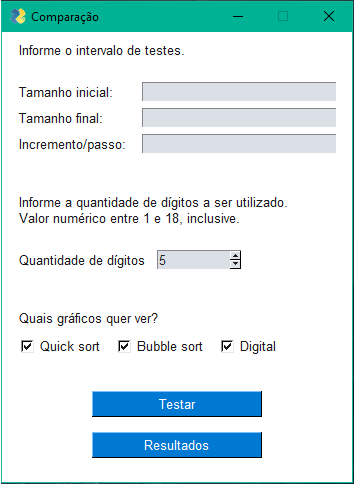
\includegraphics[width=.5\textwidth]{images/interface.png}
	\label{fig:interface}
\end{figure}

Após as escolhas dos valores, clicando no botão \textit{Testar}, o algoritmo começa a executar as devidas ordenações. Os valores obtidos são armazenados em arquivo com extensão csv (\textit{comma-separated-values}, valores separados por vírgula), e uma nova janela será aberta com o gráfico gerado a partir dos valores. Caso um novo teste seja realizado, os novos valores serão armazenados no arquivo, e o gráfico será gerado a partir da média dos mesmos. Caso já existam valores de testes, é possível clicar no botão \textit{Resultados} para visualizar o gráfico.

\subsection{Projeto da análise experimental}

A análise dos algoritmos de ordenação faz muito sentido diante do fato que existem várias opções. A escolha deve ser estudada levando em consideração aspectos como tempo de execução (algoritmo mais rápido) e espaço utilizado (algoritmo que utiliza menos recursos, como memória). Assim, toda a classes desses algoritmos é investigada a fim de se encontrar a melhor escolha possível. \cite{projeto:99}

Existem algumas formas de se determinar o custo da execução do algoritmo. A análise experimental, em particular, utilizada a execução do programa em um computador real, podendo medir o tempo de execução diretamente. Porém, esses resultados podem variar de acordo com fatores externos, como o poder computacional da máquina utilizada e sua sobrecarga, assim como a escolha do compilador. Dessa forma, os resultados de análises experimentais, em parte, não devem ser generalizados. \cite{projeto:99}

O valor do custo de execução de um algoritmo depende, principalmente, do tamanho da instância dos dados de entrada. Na caso dos algoritmos de ordenação, a distribuição dos dados também afeta o desempenho. A ordenação de um vetor parcialmente ordenado tende a ser menos custosa do ponto de vista computacional, cenário o qual denominamos de \textbf{melhor caso}. \cite{projeto:99}

Para essa análise, foram escolhidos valores altos para o tamanho da entrada, variando, para todos, a quantidade de dígitos dos números. Isso se deve ao fato de que, atualmente, possuímos um grande poder computacional, conseguindo realizar as operações de forma rápida, fazendo com que instâncias pequenas gerem resultados pouco significativos. 

\section{Resultados}

A primeira decisão tomada seria a de executar três vezes o mesmo teste para 5, 10 e 15 dígitos, onde o tamanho da entrada iria varia de 10.000 até 1.000.000, com passo de 10.000, totalizando 100 ordenações por teste para cada algoritmo. Todavia, esse modelo foi desconsiderado devido ao alto tempo de execução, principalmente do algoritmo \textit{Bubble sort}. O teste foi abortado na septuagésima quinta (75ª) ordenação, momento no qual o \textit{bubble sort} demorou, aproximadamente, 30 minutos para ser finalizado. O resultado final pode ser observado na \autoref{fig:cb_5_750k}.

\begin{figure}[h]
	\centering
	\caption{Resultado de 75 ordenações para 5 dígitos}
	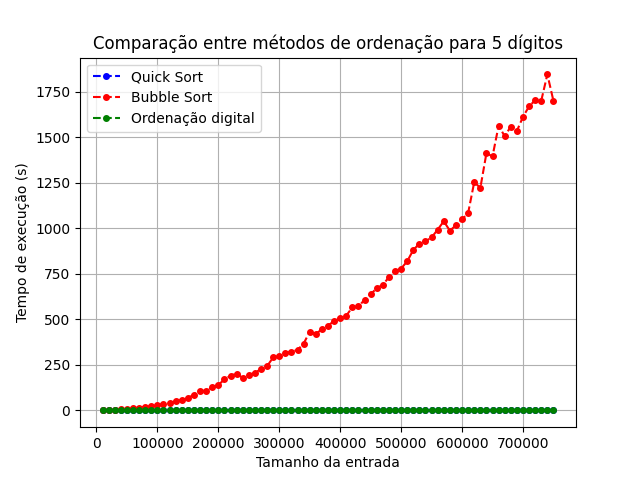
\includegraphics[width=.8\textwidth]{images/cb_5_750k.png}
	\label{fig:cb_5_750k}
\end{figure}

Como pode ser observado pelo gráfico da \autoref{fig:cb_5_750k}, a plotagem dos resultados do \textit{bubble sort} é muito superior em relação aos outros algoritmos, dificultando, inclusive, a comparação entre eles. Porém, já é possível validar o comportamento quadrático do mesmo. A \autoref{fig:sb_5_750k} mostra os valores apenas do \textit{quick sort} e do algoritmo de ordenação digital. Como foi realizado apenas um teste, pode-se observar que existem momentos que o tempo de execução aumenta em uma taxa muito alta. Isso pode ter ocorrido devido a sobrecarga de uso da máquina no momento do teste, entre outros fatores.

\begin{figure}[h]
	\centering
	\caption{Resultado de 75 ordenações para 5 dígitos (exceto \textit{bubble sort})}
	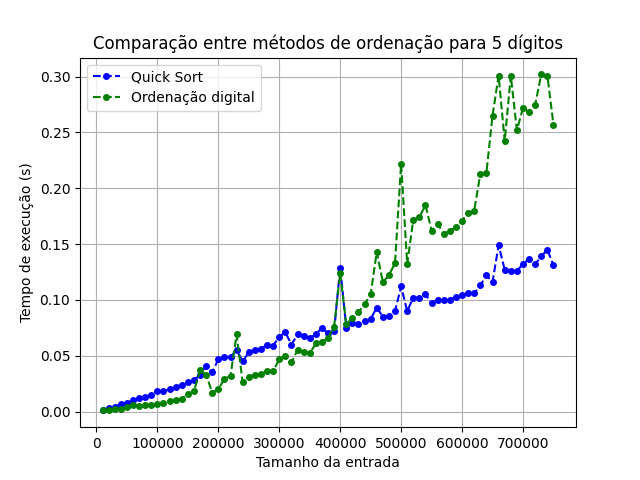
\includegraphics[width=.8\textwidth]{images/sb_5_750k.png}
	\label{fig:sb_5_750k}
\end{figure}

Diante do problema do tempo de execução, a estratégia adotada foi realizar os testes para tamanhos de entrada variando entre 10.000 e 500.000, com passo de 10.000. Os três algoritmos foram testados três vezes. Porém, para obter resultados melhores, outros sete testes foram realizados apenas com o \textit{quick sort} e o algoritmo de ordenação digital.

A figura \autoref{fig:5_500k} mostra os resultados obtidos para um total de 150 ordenações realizadas para 5 dígitos. A figura \autoref{fig:cb_5_500k} possui a plotagem dos resultados dos três algoritmos, porém, o \textit{bubble sort} possui valores muito elevados, dificultando a comparação entre os algoritmos. Como exemplo, a última ordenação (para 500.000 elementos) durou aproximadamente 14 minutos. Para melhor visualização, a \autoref{fig:sb_5_500k} mostra as plotagens para \textit{quicksort} e para o algoritmo de ordenação digital.   

\begin{figure}[]
	\centering
	\caption{Três testes para 5 dígitos}
	\begin{subfigure}[H]{0.8\textwidth}
		\centering
		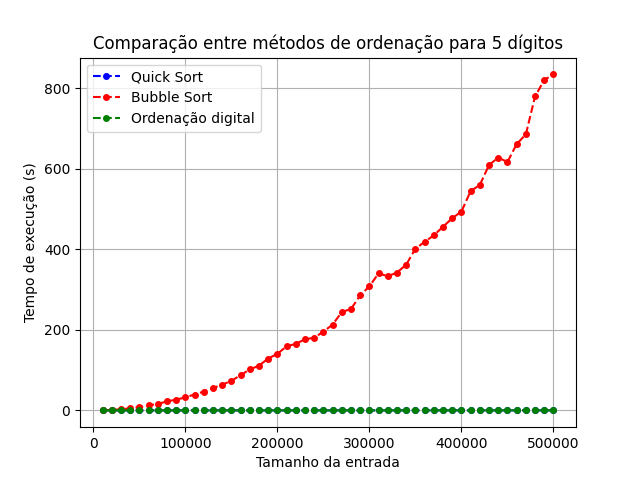
\includegraphics[width=1\textwidth]{images/cb_5_500k.png}
		\caption{com \textit{bubble sort}}
		\label{fig:cb_5_500k}
	\end{subfigure}
	\begin{subfigure}[H]{0.8\textwidth}
		\centering
		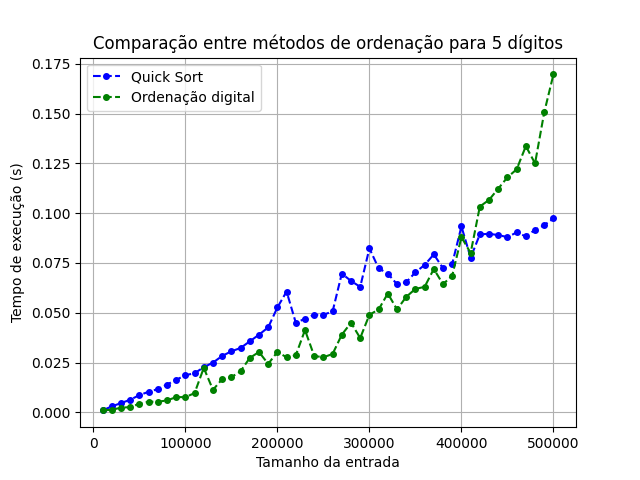
\includegraphics[width=1\textwidth]{images/sb_5_500k.png}
		\caption{sem \textit{bubble sort}}
		\label{fig:sb_5_500k}
	\end{subfigure}
	\label{fig:5_500k}
\end{figure}

A \autoref{fig:sb_otz_5_500k} mostra uma melhor aproximação do comportamento dos algoritmos em relação ao tempo de execução, devido a realização de mais testes e obtendo os resultados a partir da média. Como dito anteriormente, essa estratégia foi adotada com a intenção de reduzir as interferências de outros fatores, como por exemplo a sobrecarga de uso da máquina. Pode-se observar que a ordenação digital possui uma leve vantagem em relação ao \textit{quick sort} para até 400.000 elementos, quando o algoritmo passa a ter taxa de crescimento e tempo de execução maiores.

\begin{figure}[h]
	\centering
	\caption{Dez testes para 5 dígitos}
	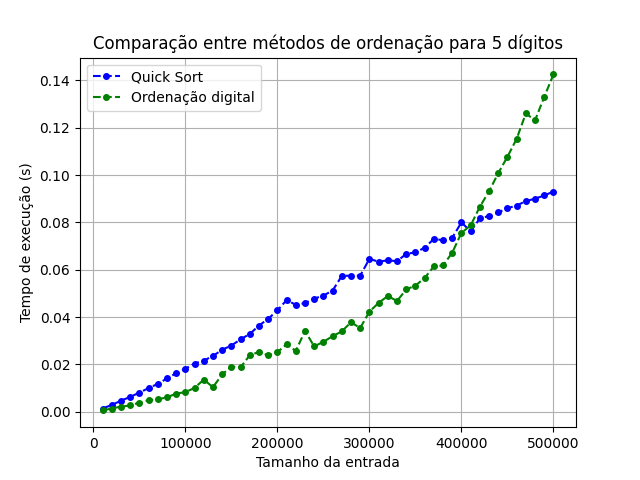
\includegraphics[width=.8\textwidth]{images/sb_otz_5_500k.png}
	\label{fig:sb_otz_5_500k}
\end{figure}

A figura \autoref{fig:10_500k} mostra os resultados obtidos para as 150 ordenações realizadas para 10 dígitos (uma melhor aproximação está na \autoref{fig:sb_otz_10_500k}). 

\begin{figure}[h!]
	\centering
	\caption{Dez testes para 10 dígitos}
	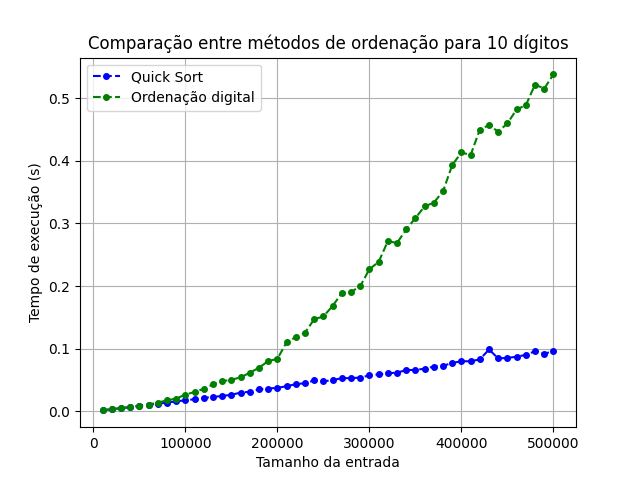
\includegraphics[width=.8\textwidth]{images/sb_otz_10_500k.png}
	\label{fig:sb_otz_10_500k}
\end{figure}

A partir desse momento, pode-se observar uma maior diferença entre os tempos de execução para os algoritmos \textit{quick sort} e ordenação digital. Em geral, o \textit{quick sort} não possui uma grande dependência com a quantidade de dígitos dos números (ou a quantidade de caracteres das palavras), onde sua complexidade de tempo de execução, em caso médio, é dada por O(n.log(n)). A ordenação digital, por sua vez, apresenta uma maior dependência da quantidade de dígitos \textit{d}, onde sua complexidade é dada por O(d.n).

\begin{figure}[]
	\centering
	\caption{Três testes para 10 dígitos}
	\begin{subfigure}[H]{0.8\textwidth}
		\centering
		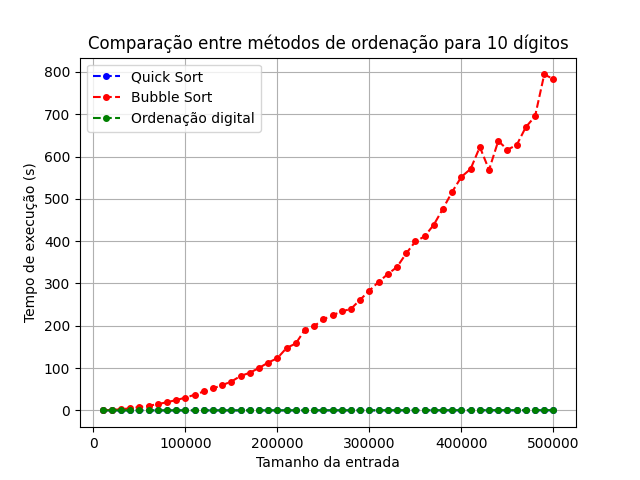
\includegraphics[width=1\textwidth]{images/cb_10_500k.png}
		\caption{com \textit{bubble sort}}
		\label{fig:cb_10_500k}
	\end{subfigure}
	\hfill
	\begin{subfigure}[H]{0.8\textwidth}
		\centering
		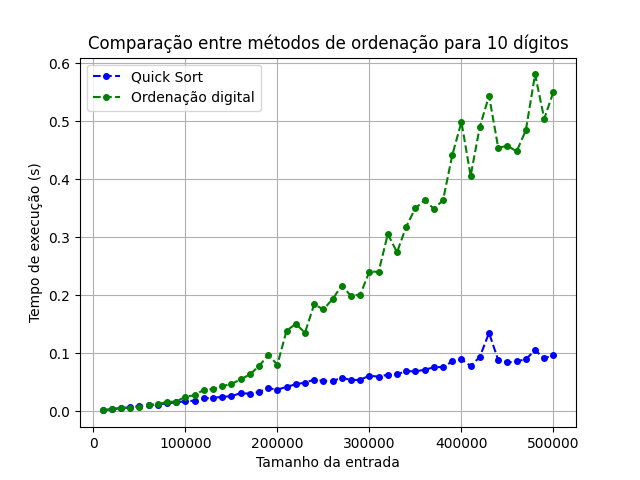
\includegraphics[width=1\textwidth]{images/sb_10_500k.png}
		\caption{sem \textit{bubble sort}}
		\label{fig:sb_10_500k}
	\end{subfigure}
	\label{fig:10_500k}
\end{figure}



A figura \autoref{fig:15_500k} mostra os resultados obtidos para as 150 ordenações realizadas para 15 dígitos (uma melhor aproximação está na \autoref{fig:sb_otz_15_500k}). Ao utilizarmos números com 15 dígitos é ainda mais fácil perceber a diferença de desempenho entre o \textit{quick sort} e o algoritmo de ordenação digital. Para valores pequenos do tamanho da entrada \textit{n} os algoritmos possuem um desempenho similar. Porém, a partir de 200.000 elementos, aproximadamente, o tempo de execução da ordenação digital cresce em uma taxa mais alta.

\begin{figure}[]
	\centering
	\caption{Três testes para 15 dígitos}
	\begin{subfigure}[H]{0.8\textwidth}
		\centering
		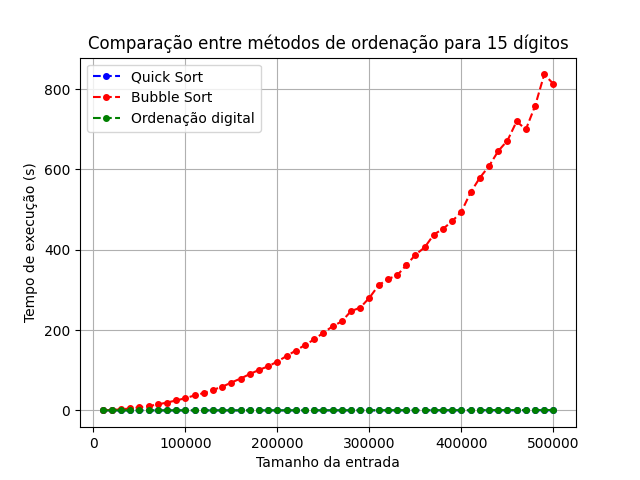
\includegraphics[width=1\textwidth]{images/cb_15_500k.png}
		\caption{com \textit{bubble sort}}
		\label{fig:cb_15_500k}
	\end{subfigure}
	\hfill
	\begin{subfigure}[H]{0.8\textwidth}
		\centering
		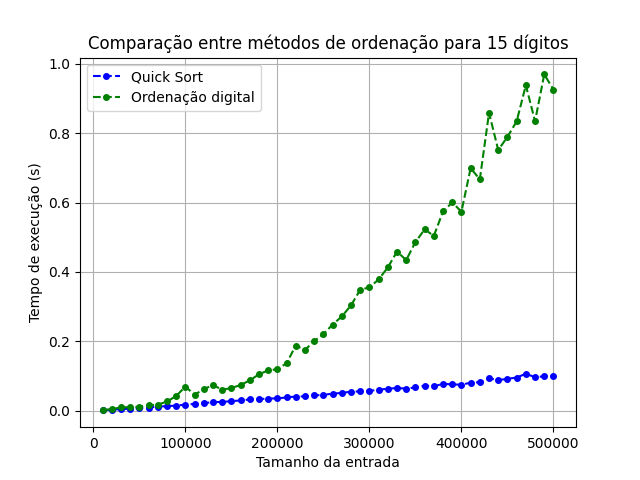
\includegraphics[width=1\textwidth]{images/sb_15_500k.png}
		\caption{sem \textit{bubble sort}}
		\label{fig:sb_15_500k}
	\end{subfigure}
	\label{fig:15_500k}
\end{figure}

\begin{figure}[h]
	\centering
	\caption{Dez testes para 15 dígitos}
	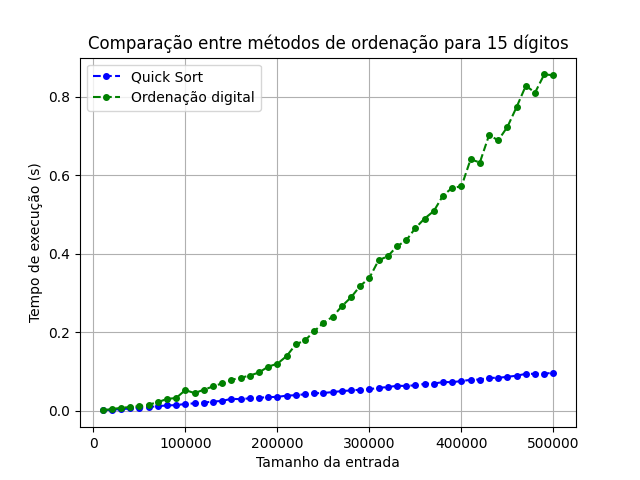
\includegraphics[width=.8\textwidth]{images/sb_otz_15_500k.png}
	\label{fig:sb_otz_15_500k}
\end{figure}

Os resultado obtido até aqui já revelam que o desempenho do algoritmo de ordenação digital depende da quantidade de dígitos dos elementos. Porém, apenas por validação, foram realizados mais três testes para 2 dígitos, onde o tamanho do conjunto varia de 10.000 até 1.000.000, com passo de 10.000. O resultado obtido está representado na \autoref{fig:sb_otz_2_1kk}. Como a quantidade de dígitos é baixa, pode-se observar um melhor desempenho do algoritmo de ordenação por dígitos, superando levemente o \textit{quick sort}. 

\begin{figure}[h!]
	\centering
	\caption{Três testes para 2 dígitos}
	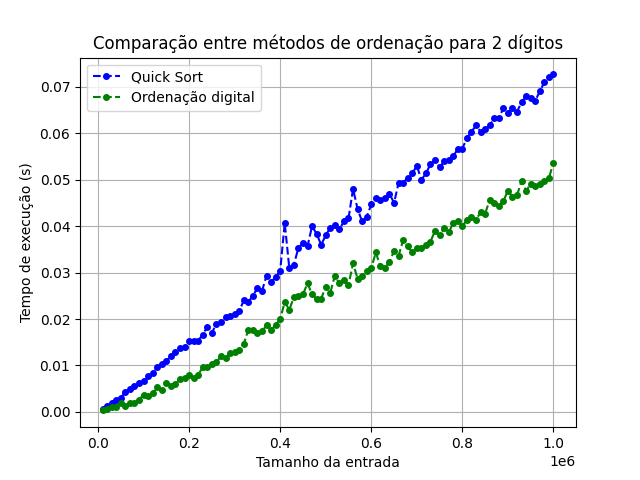
\includegraphics[width=.8\textwidth]{images/sb_otz_2_1kk.png}
	\label{fig:sb_otz_2_1kk}
\end{figure}

\section{Conclusão}

A análise e projeto de algoritmos se mostra muito importante para o desenvolvimento de sistemas ainda mais eficientes. Assim, devem ser realizadas as análises teóricas e experimentais. A análise experimental, em particular, utiliza os tempos coletados a partir da execução do algoritmo em um computador real. Porém, como existe a dependência do poder computacional, da sobrecarga de recursos no momento do teste e do compilador escolhido, os resultados não devem ser generalizados para todos os \textit{hardwares}.

O \textit{Bubble sort} é um algoritmo de ordenação estável que possui uma implementação muito simples. Os testes realizados validam o comportamento quadrático desse algoritmo em caso médio. Um algoritmo que possui complexidade de tempo de execução quadrática é considerado lento, visto que para uma base de dados grande o seu tempo de execução será muito elevado. O alto tempo de execução do \textit{bubble sort} foi validado pelos vários testes realizados nesta análise, onde para 750.000 elementos, por exemplo, o algoritmo levou aproximadamente 30 minutos para finalizar.

Os algoritmos \textit{Quick sort} e ordenação digital possuem um melhor desempenho para o tempo de execução. O segundo algoritmo, em particular, possui uma complexidade dependente da quantidade de dígitos (ou caracteres) dos elementos da base de dados. Os testes realizados validam esse dependência, onde um conjunto de dados grande que possui números com bastante dígitos eleva o tempo de execução desse algoritmo. O \textit{Quick sort}, por sua vez, não possui uma dependência direta à quantidade de dígitos. O desempenho desse algoritmo depende, principalmente, do tamanho do conjunto a ser ordenado e de uma boa implementação para que a escolha do pivô seja a melhor possível. Os testes validam o comportamento sólido do \textit{quick sort} para diferentes quantidade de dígitos e tamanhos de entrada. Esse algoritmo, portanto, é uma das melhores opções de ordenação para a maioria dos casos, determinando, inclusive, o limite inferior de tempo de execução para algoritmos de ordenação por comparação entre chaves, ou seja, para casos médios, esse algoritmo possui o menor tempo de execução possível. 

\bibliographystyle{sbc}
\bibliography{referencias.bib}

\section*{Anexo}

\href{https://github.com/MarcosKrul/analise-experimental-ordenacao}{Link do repositório contendo todo o código.}

\end{document}
